% Template for ICASSP-2010 paper; to be used with:
%          mlspconf.sty  - ICASSP/ICIP LaTeX style file adapted for MLSP, and
%          IEEEbib.bst - IEEE bibliography style file.
% --------------------------------------------------------------------------
\documentclass{article}
\bibliographystyle{plain}

% use Times
\usepackage{times}
% For figures
\usepackage{graphicx} % more modern
%\usepackage{epsfig} % less modern
\usepackage{subfigure} 
% For algorithms
\usepackage{algorithm}
\usepackage{algorithmic}

% As of 2011, we use the hyperref package to produce hyperlinks in the
% resulting PDF.  If this breaks your system, please commend out the
% following usepackage line and replace \usepackage{icml2014} with
% \usepackage[nohyperref]{icml2014} above.
\usepackage{hyperref}

% Packages hyperref and algorithmic misbehave sometimes.  We can fix
% this with the following command.
\newcommand{\theHalgorithm}{\arabic{algorithm}}

\usepackage{color}
\usepackage{amsthm}
\usepackage{amsmath}
\usepackage{amsfonts}

\newtheorem{theo}{Theorem}
\newtheorem{prop}[theo]{Proposition}
\newtheorem{lemm}[theo]{Lemma}
\newtheorem{prof}[theo]{Proof}
\renewcommand{\theprof}{}

  
\DeclareMathOperator{\rch}{RCH_\eta}
\DeclareMathOperator{\ch}{CH}
\DeclareMathOperator{\argmin}{argmin}
\DeclareMathOperator{\argmax}{argmax}
\newcommand{\re}{\mathbb{R}}
\newcommand{\na}{\mathbb{N}}
\newcommand{\rand}{{\rm Random}}
\newcommand{\randre}{{\rm RandomReal}}
\newcommand{\red}{\mathbb{R}^d}
\newcommand{\bi}{\left\lbrace -1,1 \right\rbrace}
\newcommand{\m}{{\rm minimize}}
\newcommand{\M}{{\rm maximize}}
\newcommand{\st}{{\rm subject~ to}}
\newcommand{\ms}{R_\ominus}
\newcommand{\me}{E_\ominus }
\newcommand{\aff}{{\rm aff} }


%\address{
\begin{document}
%\fontsize{9pt}{10.8pt}\selectfont
\fontsize{10pt}{12pt}\selectfont
%\ninept
%

\title{How to Use Submodular Function Oracles }
\author{onigiri}
\date{\today}


\maketitle
\newpage


\tableofcontents

\newpage

\section{Introductions}
This is the document for Submodular Functions.
We explain how to use and create submodular function oracles.
C++ and C\# are available.

\newpage

\section{How to Use Submodular Function Oracle}
We explain about a class "SubmodularOracle" and classes which derived from the class.

\begin{figure*}[h!]\label{C++OraclePic}
{
\fontsize{10pt}{12pt}\selectfont
\centering
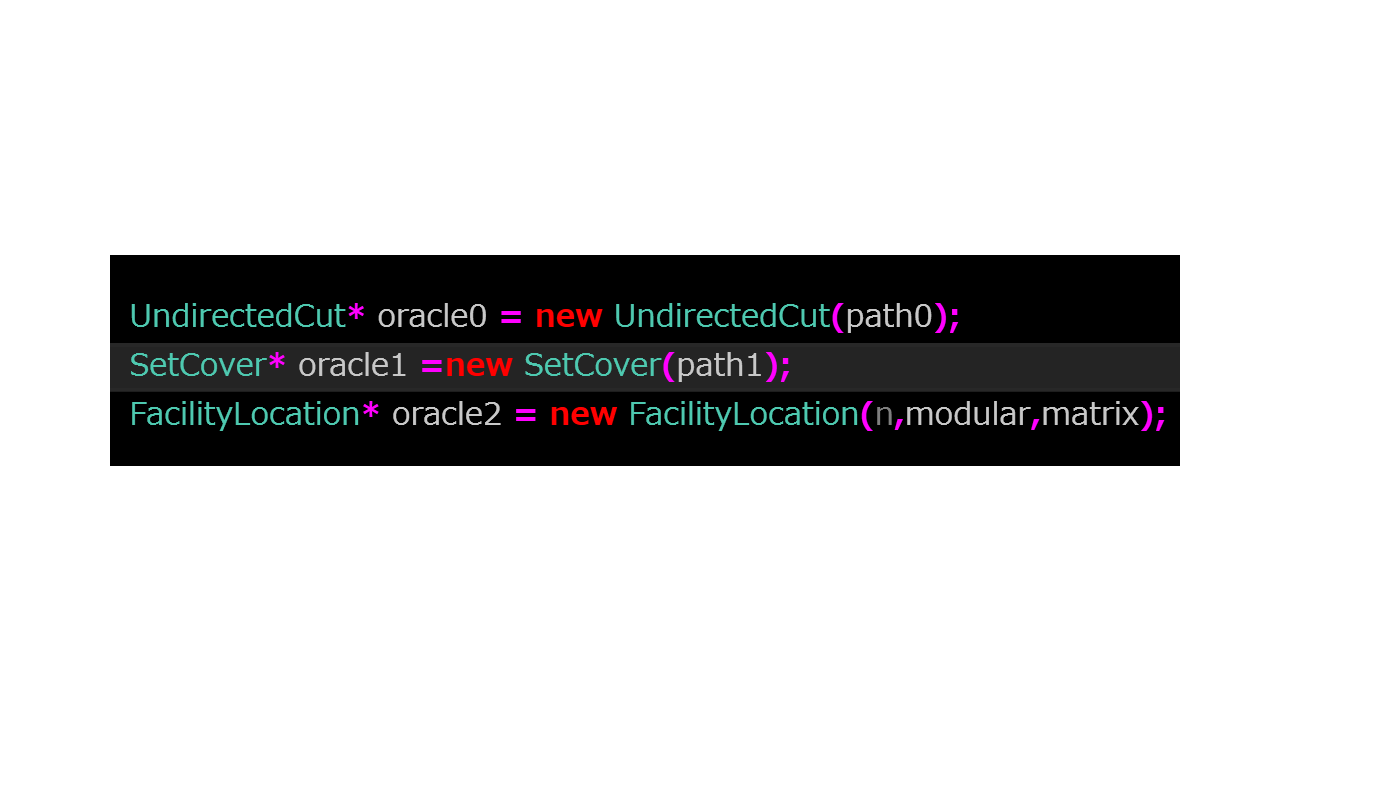
\includegraphics[height=7.0cm]{picture/C++Oracle.png}
\caption{Example of oracle by C++}
}
\end{figure*}

\begin{figure*}[h!]\label{CSOraclePic}
{
\fontsize{10pt}{12pt}\selectfont
\centering
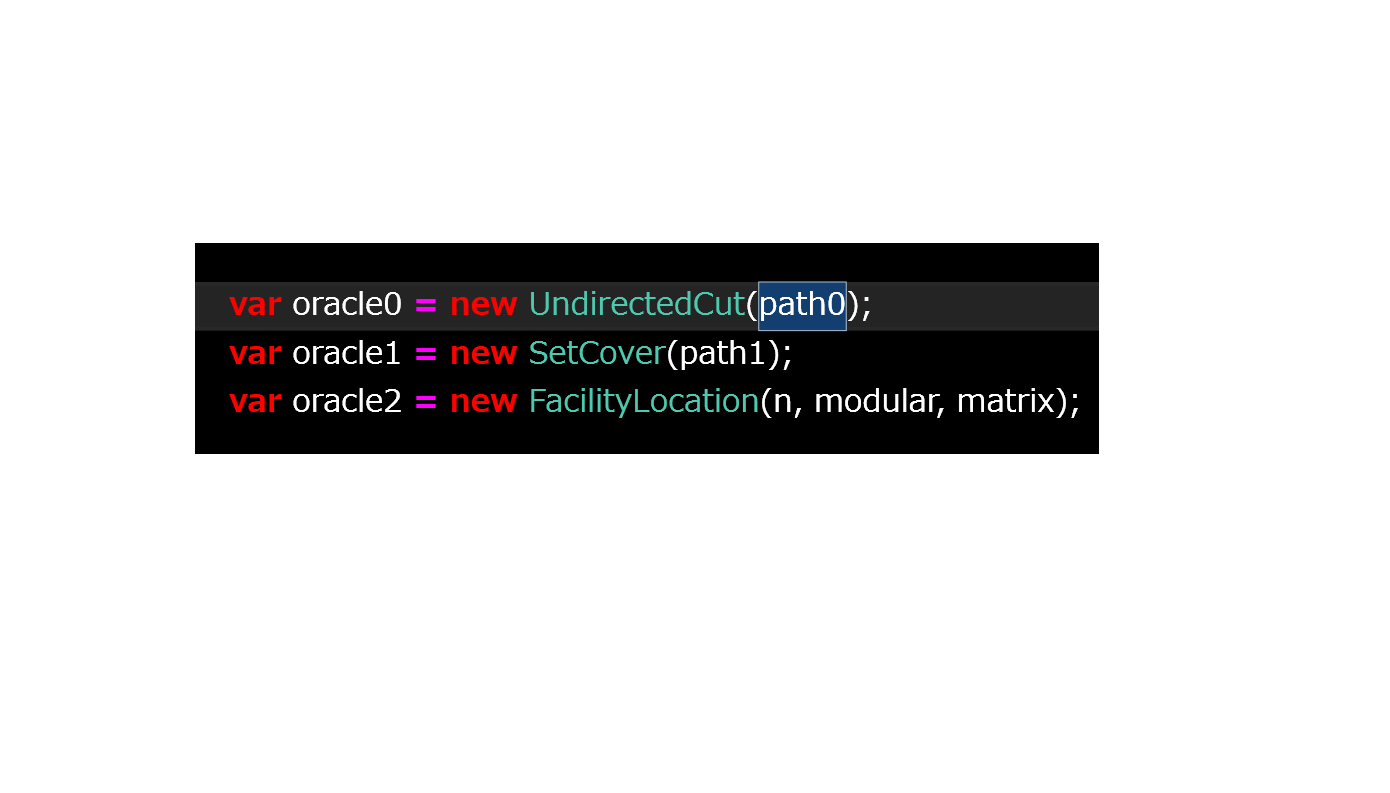
\includegraphics[height=7.0cm]{picture/CSOracle.png}
\caption{Example of oracle by C\#}
}
\end{figure*}

\subsection{Submodular Function Oracle: Base Class}\label{oracleBase}
We first explain a base class "SubmodularOracle".
This is an abstract class, therefore,
you cannot create a instance of this class.
All oracles inherit this class.

This class support methods and properties as follows.

\mbox{}

{\sf C++}
\begin{itemize}
\item int N();
\item double CalcValue(const int* order, int cardinality);
\item void CalcBase(const int* order,double* base);
\item bool IsSubmodular();
\item static void GetOrder(int $n$, int mask,int \&usedBit,int* order);
\item static void GetOrder(int $n$, string \&minimizer,int \&usedBit,int* order);
\end{itemize}

\mbox{}

{\sf C\#}
\begin{itemize}
\item int N;
\item double CalcValue(int[] order, int cardinality);
\item double[] CalcBase(int[] order);
\item bool IsSubmodular();
\item static int[] GetOrder(int $n$,int mask,out int usedBit);
\item static int[] GetOrder(string mask,out int usedBit)
\end{itemize}


\mbox{}

{\sf details}
\begin{itemize}
\item N() gets the cardinality of the ground set.
\item CalcValue() calculates the value $f(X)$, where $X:=\cup _{0\leq i < {\rm cardinality}} {\rm \{ order }[i] \}$.
\item CalcBase() calculates the base according to order,
i.e., this finds the base whose ${\rm order}[i]$th element is $f(X_i)-f(X_{i-1})$,
where $X_:=\cup _{0\leq i <= i} {\rm \{order }[i] \}$.
In C++, instead of returning an array, we update the second argument base.
\item IsSubmodular() checks whether this oracle is submodular or not.
Note that it takes $O(N^2 * N^2)$ time.
\item GetOrder() is for converting a set (bitmask) to an order since our submodular function oracle need an order instead of a set.
If bitmask represents a set $X$ and we get order and usedBit by this function,
then in order to know $f(X)$, we only need to call CalcValue(order, usedBit).
We cannot decide this order uniquely.
Note that if we use integer mask, then positions is read from right to left, but if we use string mask, then positions read from left to right.
When we use string, all characters which are not '0' are seemed as '1'.
$n$ is the size of the number of positions of mask. Here, usedBit is the number of positions which is not $0$.
In C++, instead of returning an array, the argument order is updated.
\end{itemize}




\mbox{}

{\sf examples}\\ \mbox{}\\
Let oracle $f$ is a modular function on $\{ 0,1,2 \}$
which satisfies \\ $f(\{ 0 \})=10$,\\ $f(\{ 1\}) = 7$, \\ $f(\{ 2 \}) = 3$.\\
Then, N() returns $3$.\\
CalcValue($(2,0,1), 0$) returns $f(\{  \})=0$,\\
CalcValue($(2,0,1), 1$) returns $f(\{ 2 \})=3$,\\
CalcValue($(2,0,1), 2$) returns $f(\{ 2,0 \})=13$,\\
CalcValue($(2,0,1), 3$) returns $f(\{ 2,0,1 \})=20$.\\
Of course CalcBase($(2,0,1)$) returns $(13-3,20-13,3-0) = (10,7,3)$.
Let $n=5$ and mask is a integer $6$.
Then, GetOrder($n=5$, int mask, usedBit) returns order $=(1,2,4,3,0)$ and usedBit $=3$,
since $6=00110$ if we use binary expression.
Here, $4$ is the left most position and $0$ is the right most position.
It is important that $1,2$ comes before than $0,3,4$,
and orders of $1,2$ or $0,3,4$ do not matter.
If we use a string mask $" 00110" $,
then GetOrder($n=5$, string mask, usedBit) returns order $=(2,3,4,1,0)$ and usedBit $=3$.
Here, $4$ is the right most position and $0$ is the left most position.

\newpage

\subsection{Submodular Function Oracles: Derived Class}\label{oracleDrived}

We next explain about derived classes.
All these function normally does not have their own functions,
we only explain about the constructors.

There exist two type of constructors for each submodular function oracle.
One constructor needs a path of data which is created by DataCreator.
The other constructor needs variables directly.

\mbox{}

{\sf C++}
\begin{itemize}
\item NameOfDerivedClass(string path);
\item UndirectedCut(int $n$, double* modular, double** weight);
\item DirectedCut(int $n$, double* modular, double** weight);
\item ConnectedDetachment(int $n$, double* modular, map<int,bool>* edges);
\item FacilityLocation(int $n$, double* modular, double** matrix);
\item GraphicMatroid(int $n$, int V, double* modular, int* heads, int*tails);
\item BinaryMatrixRank(int $n$, int row, double* modular, bool** columnVectors);
\item NegativeSymmetricMatrixSummation(int $n$, double* modular, double** matrix);
\item SetCover(int $n$, int m, double* modular, double* weight, int* length, int** edges);
\end{itemize}

\mbox{}

{\sf C\#}
\begin{itemize}
\item NameOfDeriveClass(string path);
\item UndirectedCut(int $n$, double[]modular, double[][] weight);
\item DirectedCut(int $n$, double[]modular, double[][] weight);
\item ConnectedDetachment(int $n$, double[] modular, HashSet<int>[] edges);
\item FacilityLocation(int $n$, double[] modular, double[][] matrix);
\item GraphicMatroid(int $n$, int V, double[] modular, int[]heads, int[]tails);
\item BinaryMatrixRank(int $n$, int row, double[] modular, bool[][] columnVectors);
\item NegativeSymmetricMatrixSummation(int $n$, double[] modular, double[][] matrix);
\item SetCover(int $n$, int m,double[] modular, double[]weight, int[][] edges);
\end{itemize}


\mbox{}

{\sf details}
All the arguments $n$ above means the cardinality of the ground set
and modular means a modular function.
We explain about the other arguments.
\begin{itemize}
\item NameDeriveClass() is a standard constructor.
We need to change the name according to what we want to use.
For example, if we want to use undirected cut, we need to use UndirectedCut().
For the argument path, we need to set a path where data exists,
like ${\rm C:\backslash Submodular\backslash UndirectedCut\backslash 10\_ 8}$.
The data should be created by the DataCreator application.
\item UndirectedCut() needs a matrix "weight" which express' weight of edges.
\item DirectedCut() needs a matrix "weight" which express' weight of edges.
\item ConnectedDetachment() needs incidence list "edges" of the graph of map in C++ or of HashSet C\#.
\item FacilityLocation() needs a matrix.
\item GraphicMatroid() needs the number of cardinality "V" of a vertex set.
It also needs two array, "heads" and "tails", which express edges of the graph.
The $i$th edge is represented by \{heads[$i$], tails[$i$]\}.
\item BinaryMatrixRank() needs "row" which express the number of rows of the matrix.
The matrix is expressed by column vectors "columnVectors".
\item NegativeSymmetricMatrixSummation() need a non-positive symmetric matrix.
\item SetCover() needs the cardinality $m$ of the other set of bipartite graph,
which has weight by "weight".
It also needs incidence list "edges" of the graph.
In C++, we need "length", too.
Here, length[$i]$ represents the cardinality of edges[$i$].
\end{itemize}


\newpage
\section{How to Use Submodular Function Minimization Algorithms}
We explain about a class "SubmodularFunctionMinimization" and classes which derived from the class.

\begin{figure*}[h!]\label{C++MinPic}
{
\fontsize{10pt}{12pt}\selectfont
\centering
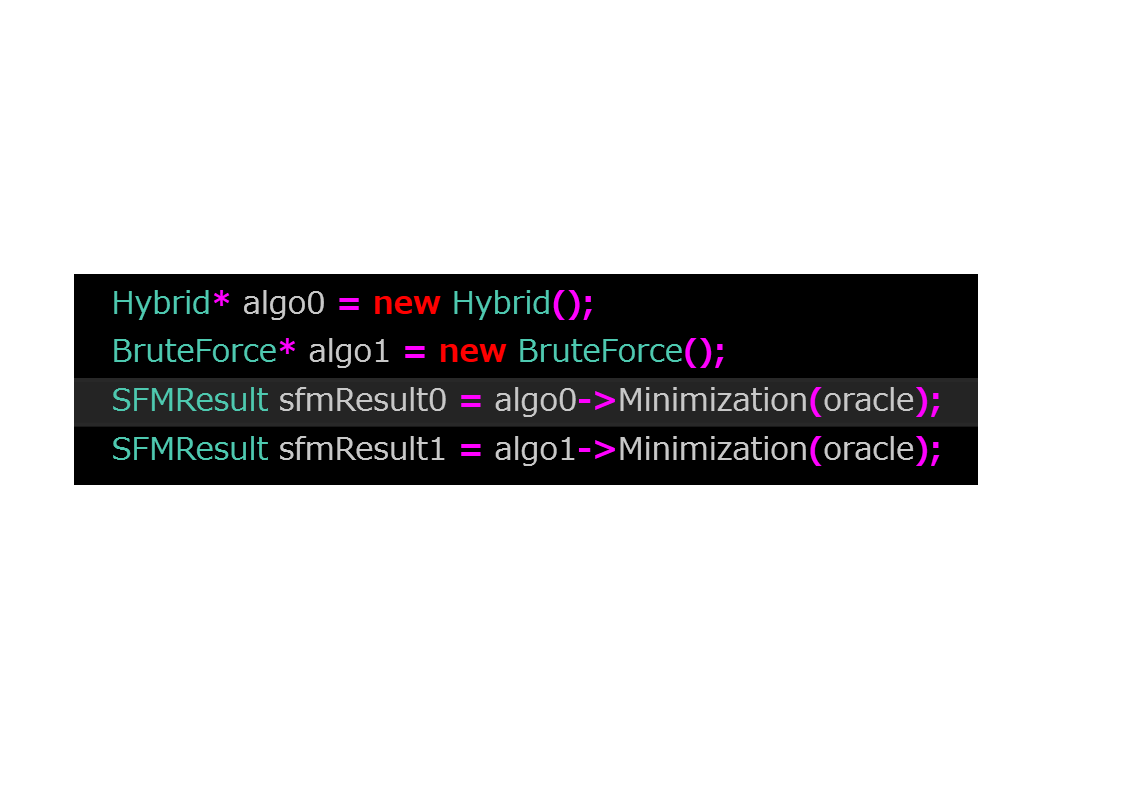
\includegraphics[height=7.0cm]{picture/C++Min.png}
\caption{Example of minimization by C++}
}
\end{figure*}

\begin{figure*}[h!]\label{CSMinPic}
{
\fontsize{10pt}{12pt}\selectfont
\centering
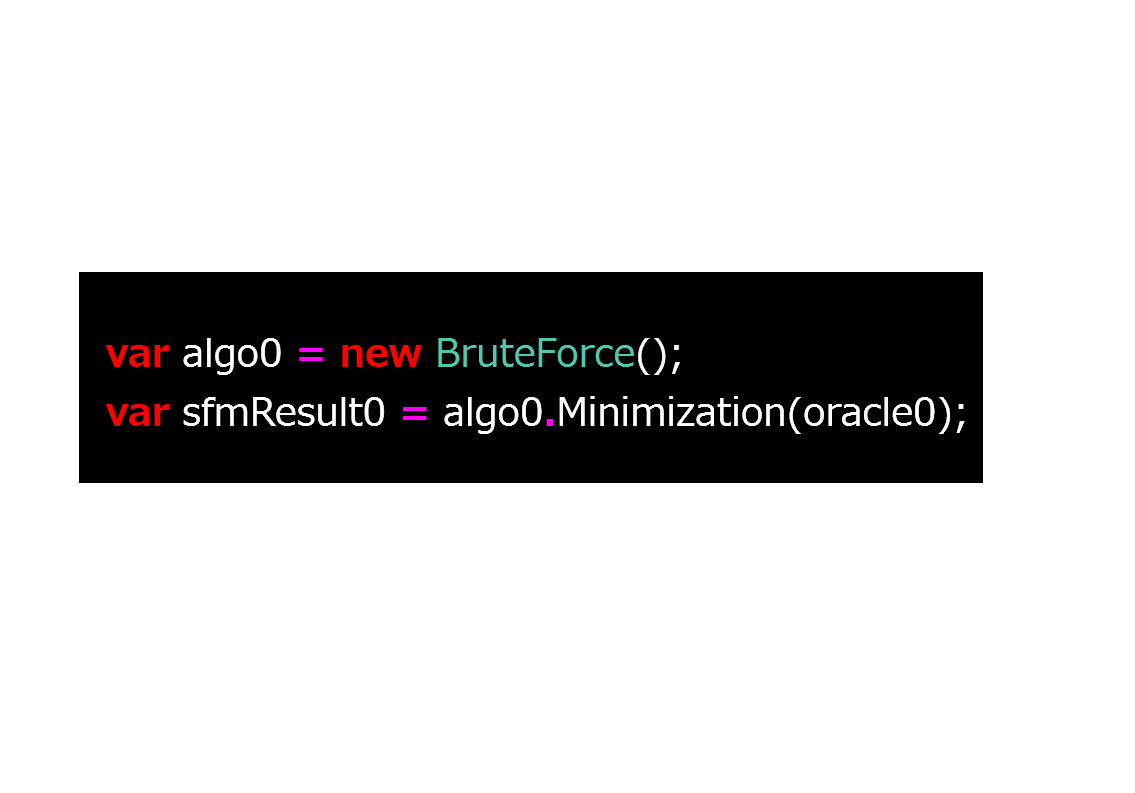
\includegraphics[height=7.0cm]{picture/CSMin.png}
\caption{Example of minimization by C\#}
}
\end{figure*}

\newpage

\subsection{Submodular Function Minimization}
SubmodularFunctionMinimization class and classes derived from it has a method SFMResult Minimization(SubmodularOracle* oracle) in C++,
and SFMResult Minimization(SubmodularOracle oracle) in C\#.
Here, SFMResult which we discuss later is a class which includes some results of execution.

If we are given a submodular function oracle,
all we have to do are to make a instance of algorithm and give it a oracle,
like Figure. \ref{C++MinPic} or Figure. \ref{CSMinPic}.


\newpage
\subsection{SFMResult Class}
We next explain about "SFMResult" class which has some information about execution results.


\mbox{}

{\sf methods}
\begin{itemize}
\item int N();
\item long Iteration();
\item long ExecutionTime();
\item long OracleTime();
\item long ReductionTime();
\item long OracleCall();
\item long BaseCall();
\item long ReductionCall();
\item double MinimumValue();
\item string Minimizer();
\item double DualValue();
\item void X(double* \&x);
\item void Output(string path, bool withX = true);
\end{itemize}

\mbox{}

Note that if we use C\#,
these functions are properties.
Hence, we do not need ().
Moreover, in C\#, X returns an array double[],
and the argument x is not required.


\mbox{}

{\sf details}
\begin{itemize}
\item int N() returns the cardinality of the ground set of the submodular function.
\item long Iteration() returns the number of iterations of the algorithm.
\item long ExecutionTime() return the total time which algorithm needed to find a minimizer.
\item long OracleTime() returns the total time which algorithm needed to calculate oracle values and bases.
\item long ReductionTime() return the total time which algorithm needed to execute Reduction().
\item long OracleCall() returns the number of oracle call in the algorithm.
\item long BaseCall() returns the number of base created in the algorithm.
\item long ReductionCall() returns the number of reduction call.
\item double MinimumValue() returns an oracle value by using above minimizer.
\item string Minimizer() returns a bitmask expression of a minimizer.
For example, if a submodular function whose cardinality of ground set is $6$
has a minimizer $\{ 0,3,4\}$,
then the returned value is "100110".
\item double DualValue() returns the objective value of dual problem with above X.
If the algorithm does not use dual formulation, then we set this value $0$.
\item void X(double* \&x) returns a feasible solution at the end of the algorithm of the dual problem.
It is not necessary to be a optimal maximizer and if the algorithm does not use dual formulation, then the returned value is NULL.
If we use CaluBase() instead of CalcValue(), then this call is not counted.
If we use ClacValue() instead of CalcBase() in order to create a base,
then this is not counted.
\item void Output(string path) writes above data to a file at path.
If we set withX = false, then x is not written to the file.
The out put is like Figure \ref{outputSFMResult}.
\end{itemize}

\begin{figure*}[h!]\label{outputSFMResult}
{
\fontsize{10pt}{12pt}\selectfont
\centering
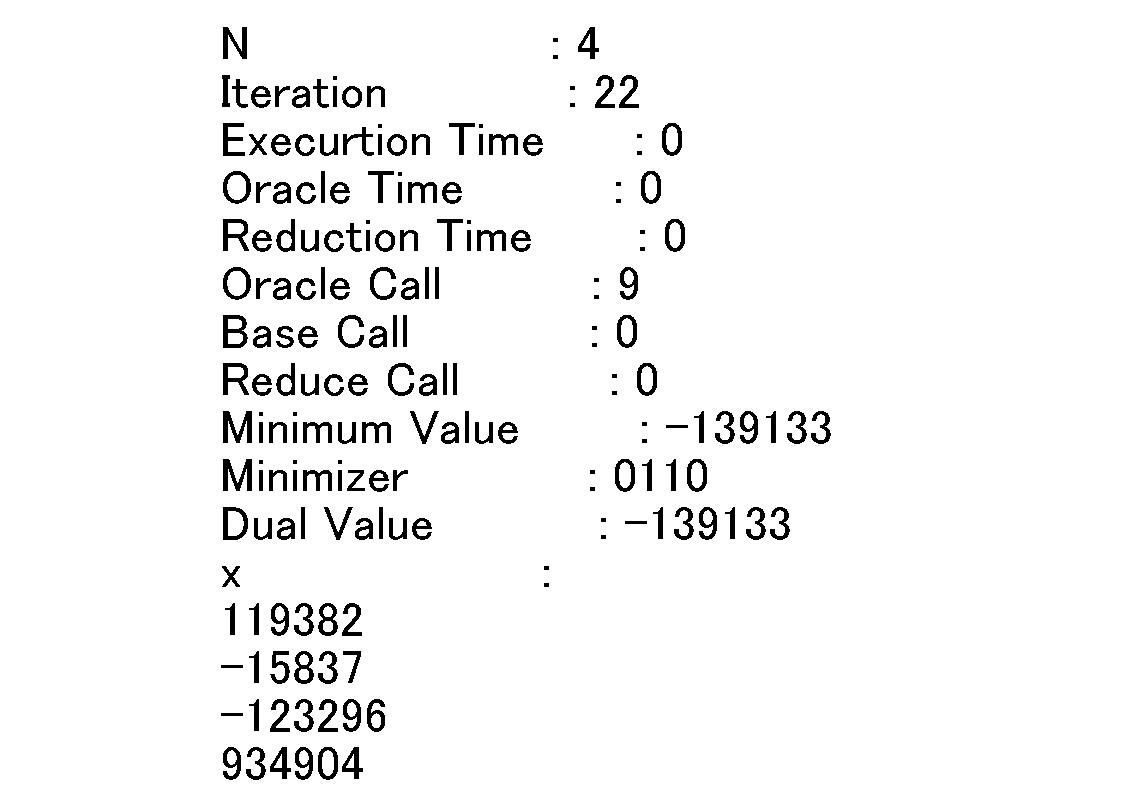
\includegraphics[height=7.0cm]{picture/SFMResult.png}
\caption{Output file by Output()}
}
\end{figure*}

\newpage
\section{How to develop Submodular Function Oracle}
We explain what to do to make submodular function oracle.
When we create a new submodular function's oracle,
please inherit a class "SubmodularOracle".
We need to implement constructor, CalcValue(), CalcBase() (optional),
and destructor (in C++).

\begin{figure*}[h!]\label{C++OracleDef}
{
\fontsize{10pt}{12pt}\selectfont
\centering
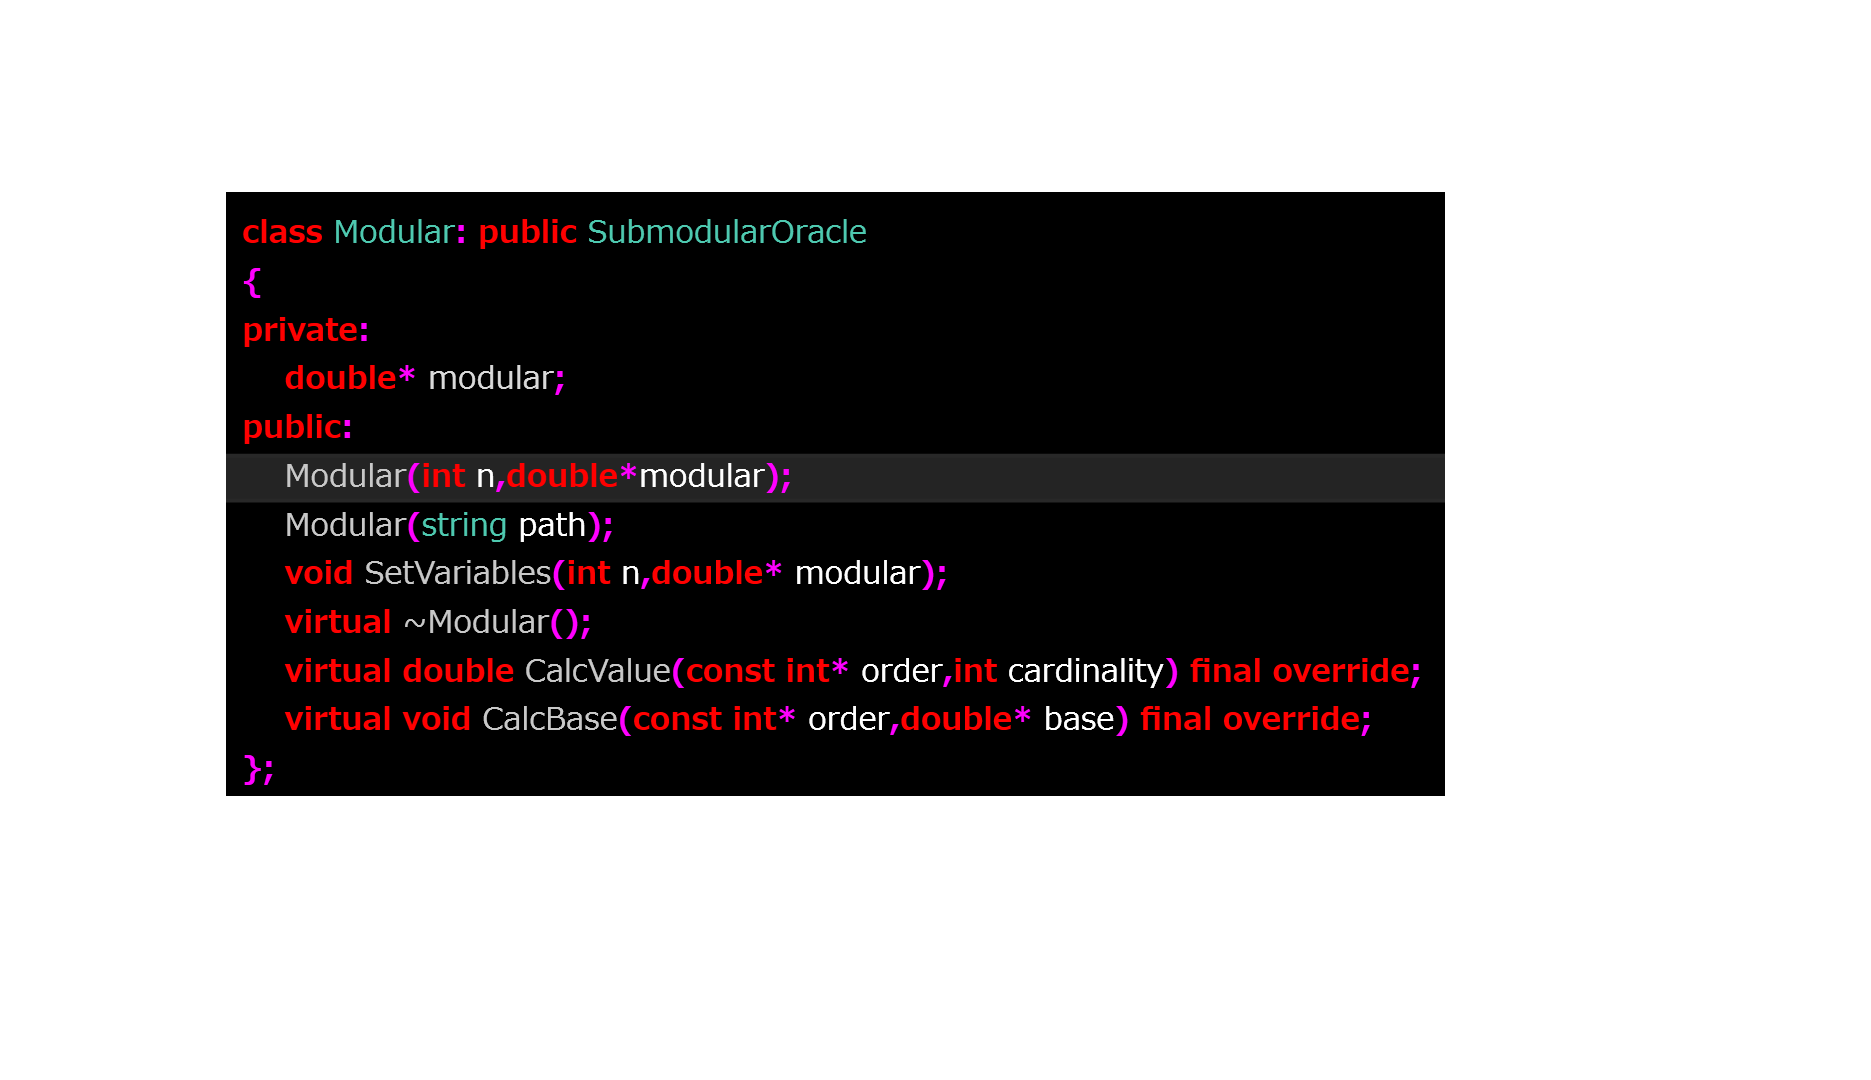
\includegraphics[height=7.0cm]{picture/C++ConstructorOracleDef.png}
\caption{Example of a header file by C++}
}
\end{figure*}



\subsection{Constructor}
We need to initialize N and fOfEmpty.
N is the cardinality of the ground set 
and fOFEmpty is the value $f(\emptyset)$, where $f$ is the submodular function.
It is possible to initialize fOfEmpty by calling CalcValue()
(in the case of Figure \ref{C++ConstOracleImp}, we do not call CalcValue()).
\begin{figure*}[h!]\label{C++ConstOracleImp}
{
\fontsize{10pt}{12pt}\selectfont
\centering
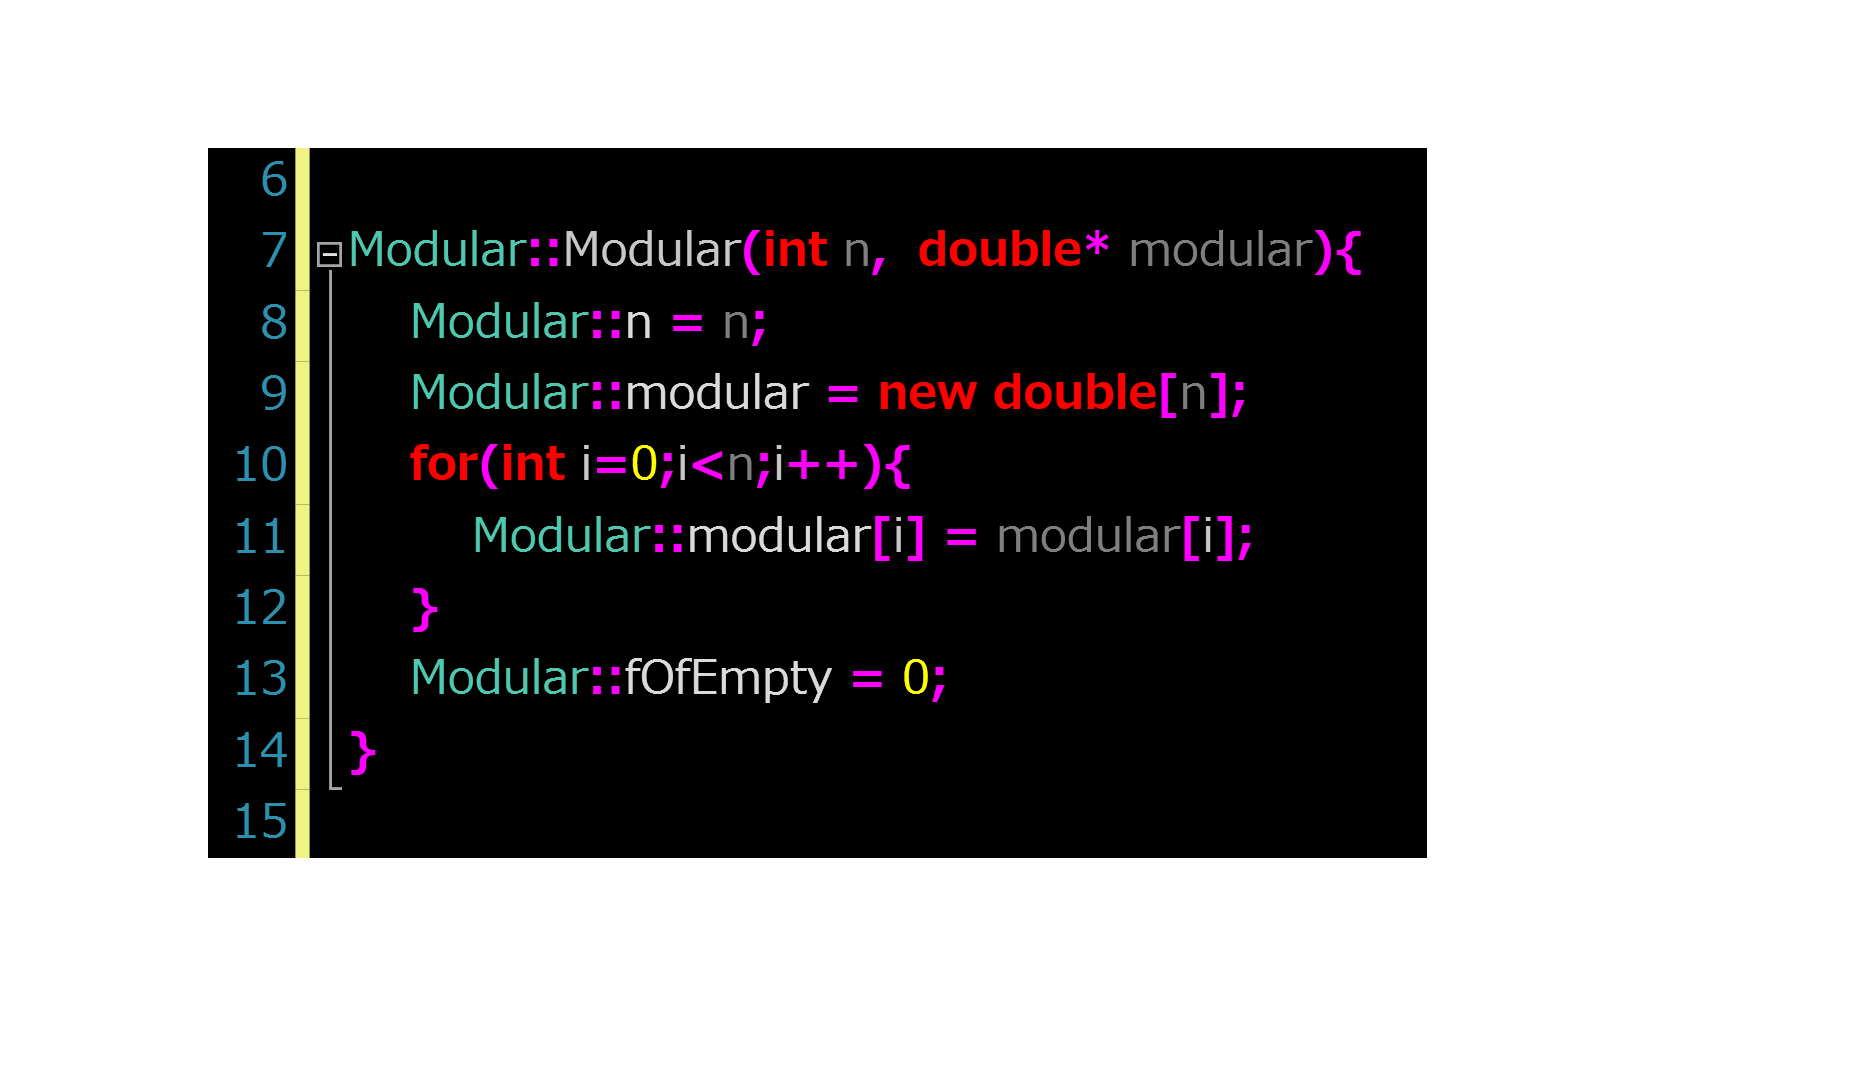
\includegraphics[height=7.0cm]{picture/C++ConstructorOracleImp.png}
\caption{The implementation for constructor of a modular function}
}
\end{figure*}

\subsection{CalcValue()}
We need to implement double CalcValue(const int* order, int cardinality) in C++
and double CalcValue(int[]order, int cardinality) in C\#.
This function calculates the oracle value.
Let $f(X)$ is a value which we want to calculate.
Then $X$ is expressed by "order" and "cardinality", i.e.,
$X$ is defined by $\cup _{0\leq i < {\rm cardinality}} {\rm order}[i]$.

For example,
a implementation for modular function is as Figure \ref{C++GetValueModular}.
\begin{figure*}[h!]\label{C++GetValueModular}
{
\fontsize{10pt}{12pt}\selectfont
\centering
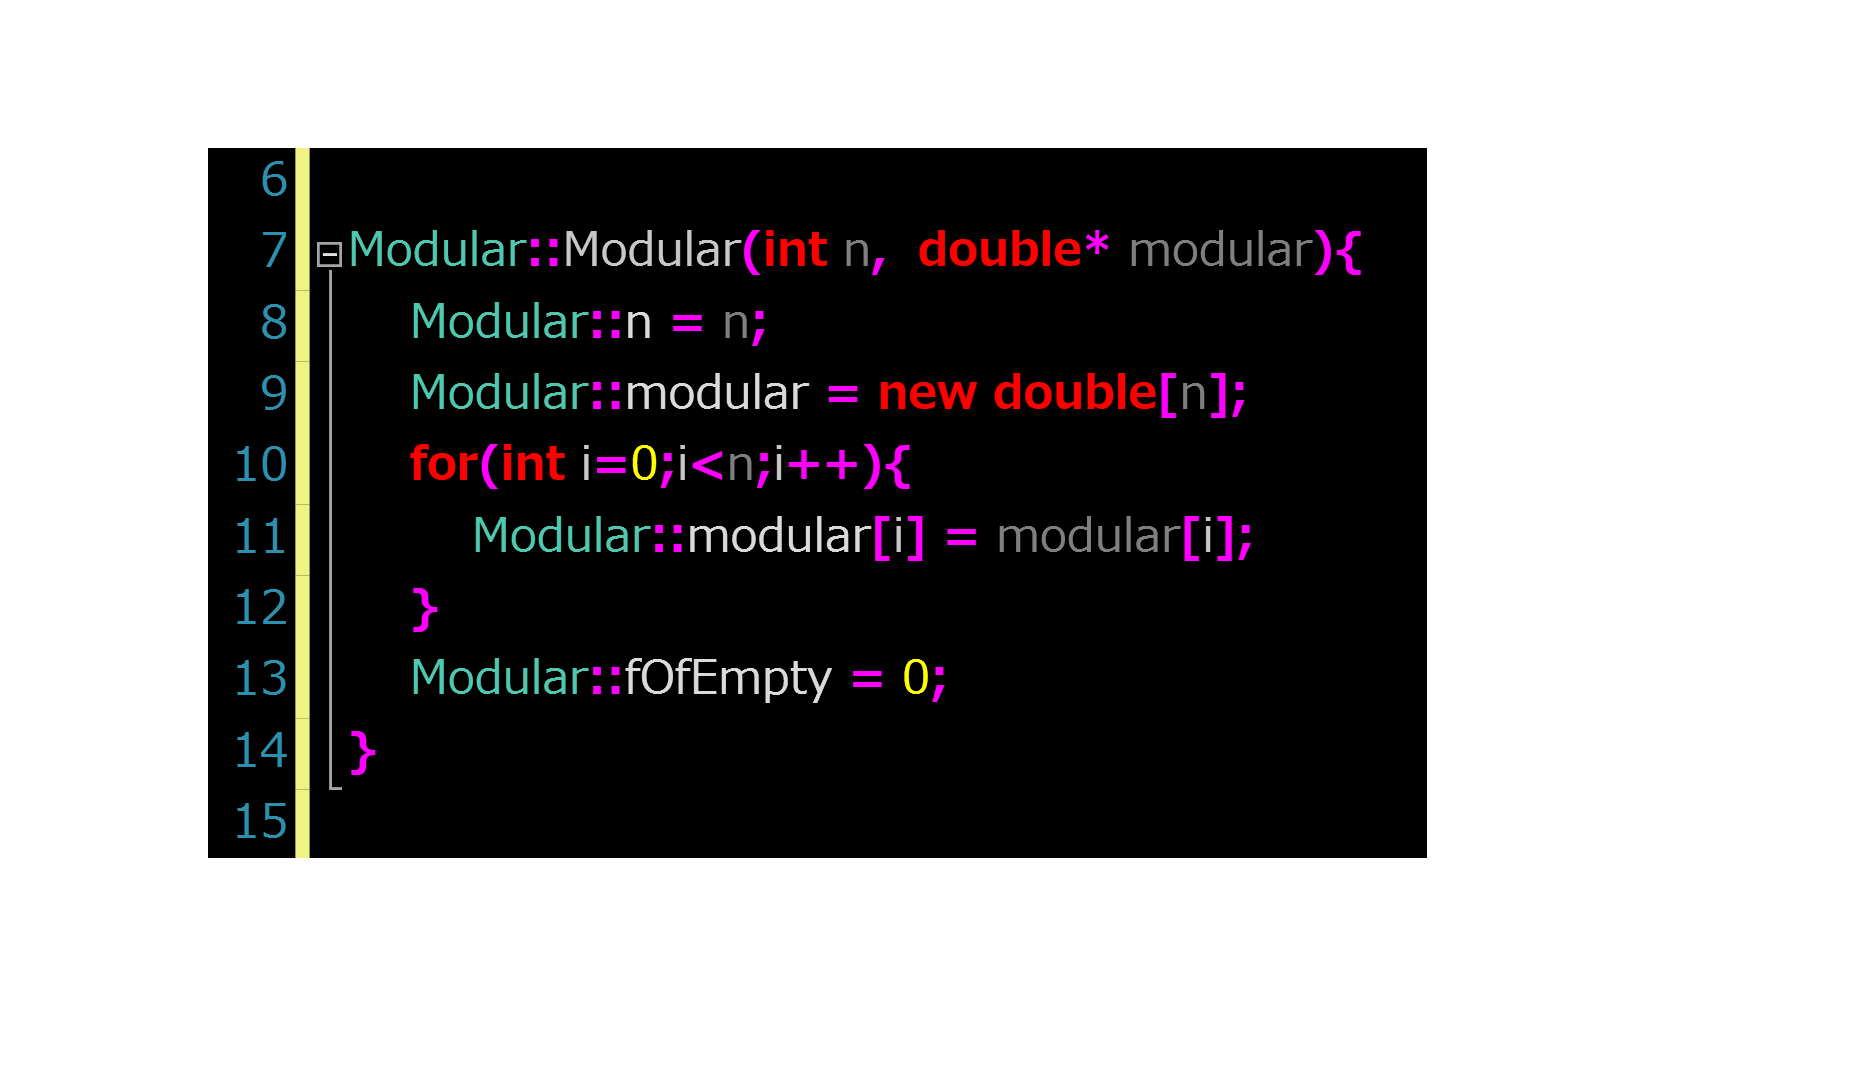
\includegraphics[height=7.0cm]{picture/C++GetValueModular.png}
\caption{The implementation for GetValue() of a modular function}
}
\end{figure*}

\subsection{CalcBase()}
This function is defined by  void CalcBase(const int* order, double* base) in C++
and double[] CalcBase(int[] order) in C\#.
This is an optional function, therefore you do not need to implement this function.
In the case that we do not implement this function,
we need to call CalcValue() for $n$ times,
where $n$ is the cardinality of the ground set.
If there exists a way to calculate a base fast,
we recommend to implement this function.
For example,
a base of modular function is defined as Figure \ref{C++CalcBaseModular} in C++ 
and as Figure \ref{CSCalcBaseModular} in C\#.

\begin{figure*}[h!]\label{C++CalcBaseModular}
{
\fontsize{10pt}{12pt}\selectfont
\centering
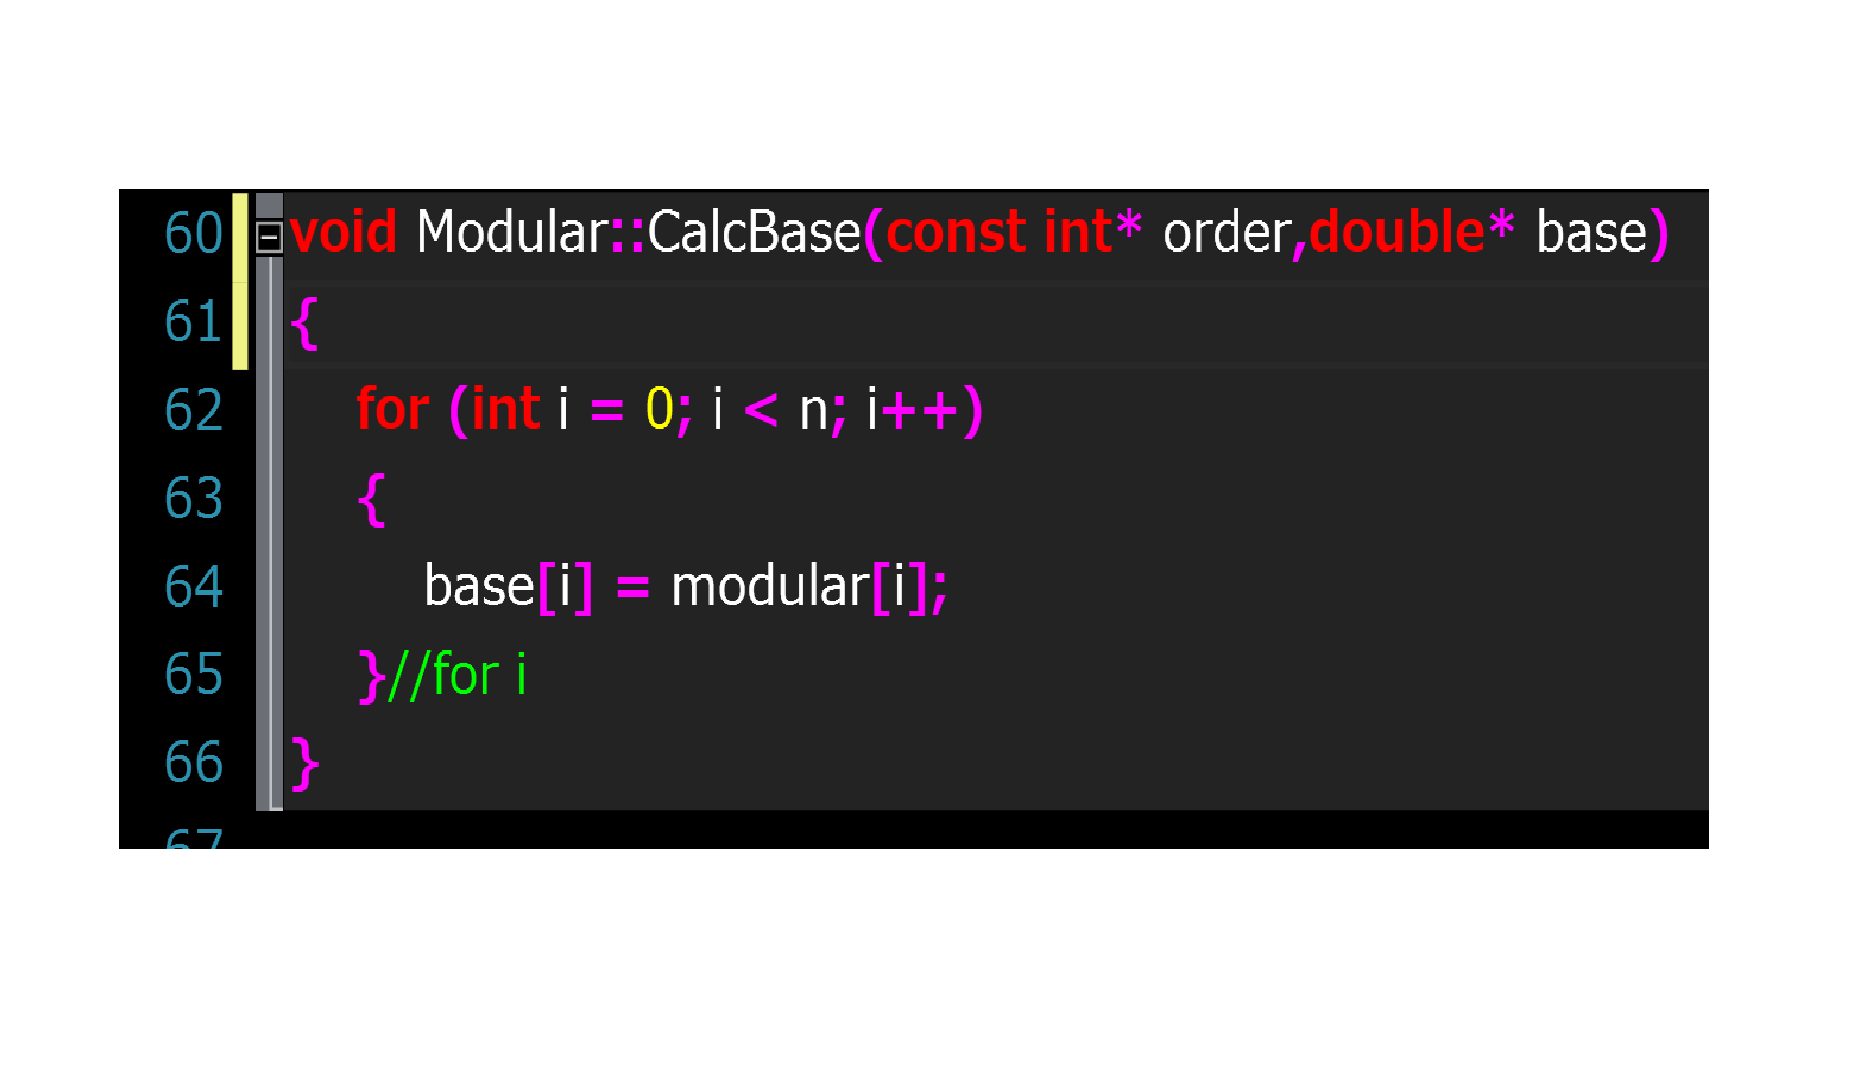
\includegraphics[height=7.0cm]{picture/C++CalcBaseModular.png}
\caption{The implementation for GetBase() of a modular function by C++}
}
\end{figure*}

\begin{figure*}[h!]\label{CSCalcBaseModular}
{
\fontsize{10pt}{12pt}\selectfont
\centering
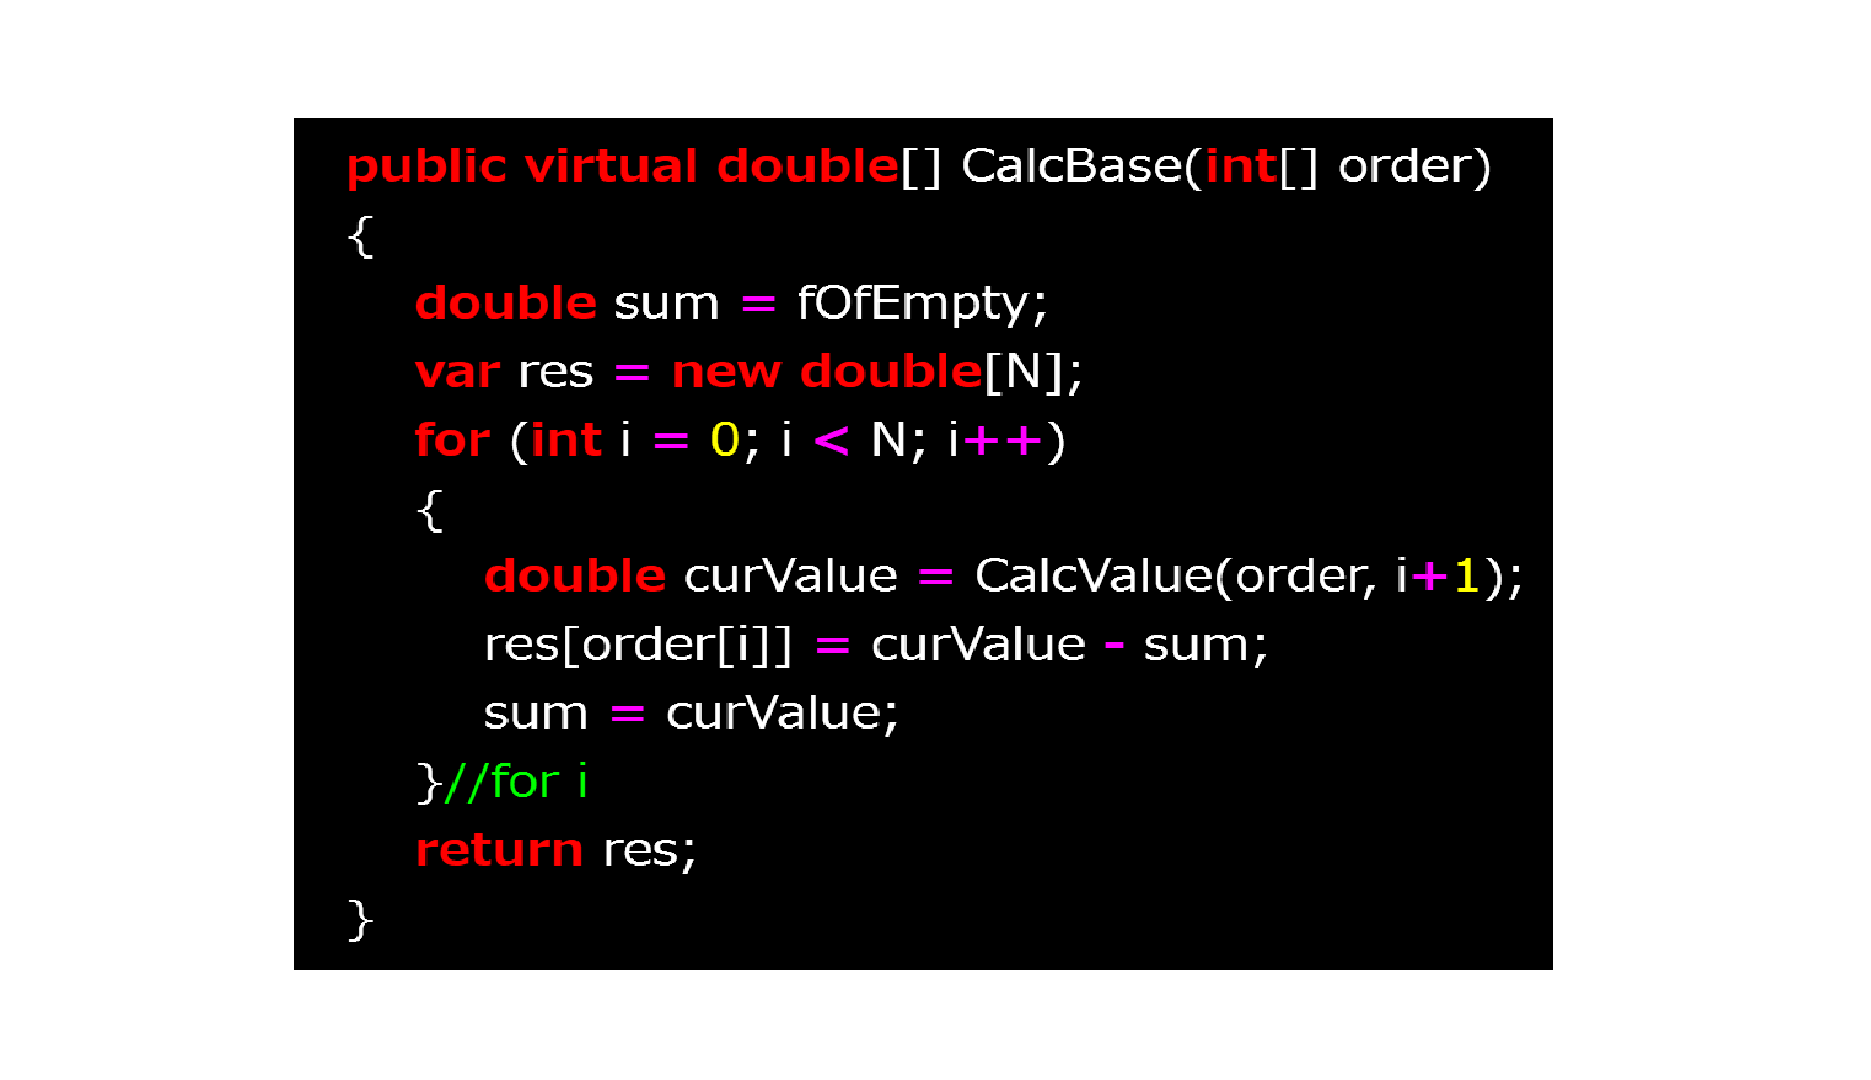
\includegraphics[height=7.0cm]{picture/CSCalcBaseModular.png}
\caption{The implementation for GetBase() of a modular function by C\#}
}
\end{figure*}


\subsection{destructor}
We need to implement destructor in C++.
Please delete what you allocate memory.



\newpage
\section{How to develop Submodular Function Minimization Algorithms}
We explain what to do to make submodular function minimization algorithm.
When we create a new submodular function's oracle,
please inherit a class "Minimization".

\subsection{Minimization()}
Any class which inherit "Minimization" class must implement
SFMResult Minimization(SubmodularOracle* oracle) in C++
and SFMResult Minimization(SubmodularOracle oracle) in C\#.
Please implement call SetOracle() at the beginning of Minimization() and
call SetResult() at the end of it.
SetOracle needs an argument and SetResult needs three or four arguments.
This function is implemented as \ref{C++Min} and \ref{CSMin}.

\begin{figure*}[h!]\label{C++Min}
{
\fontsize{10pt}{12pt}\selectfont
\centering
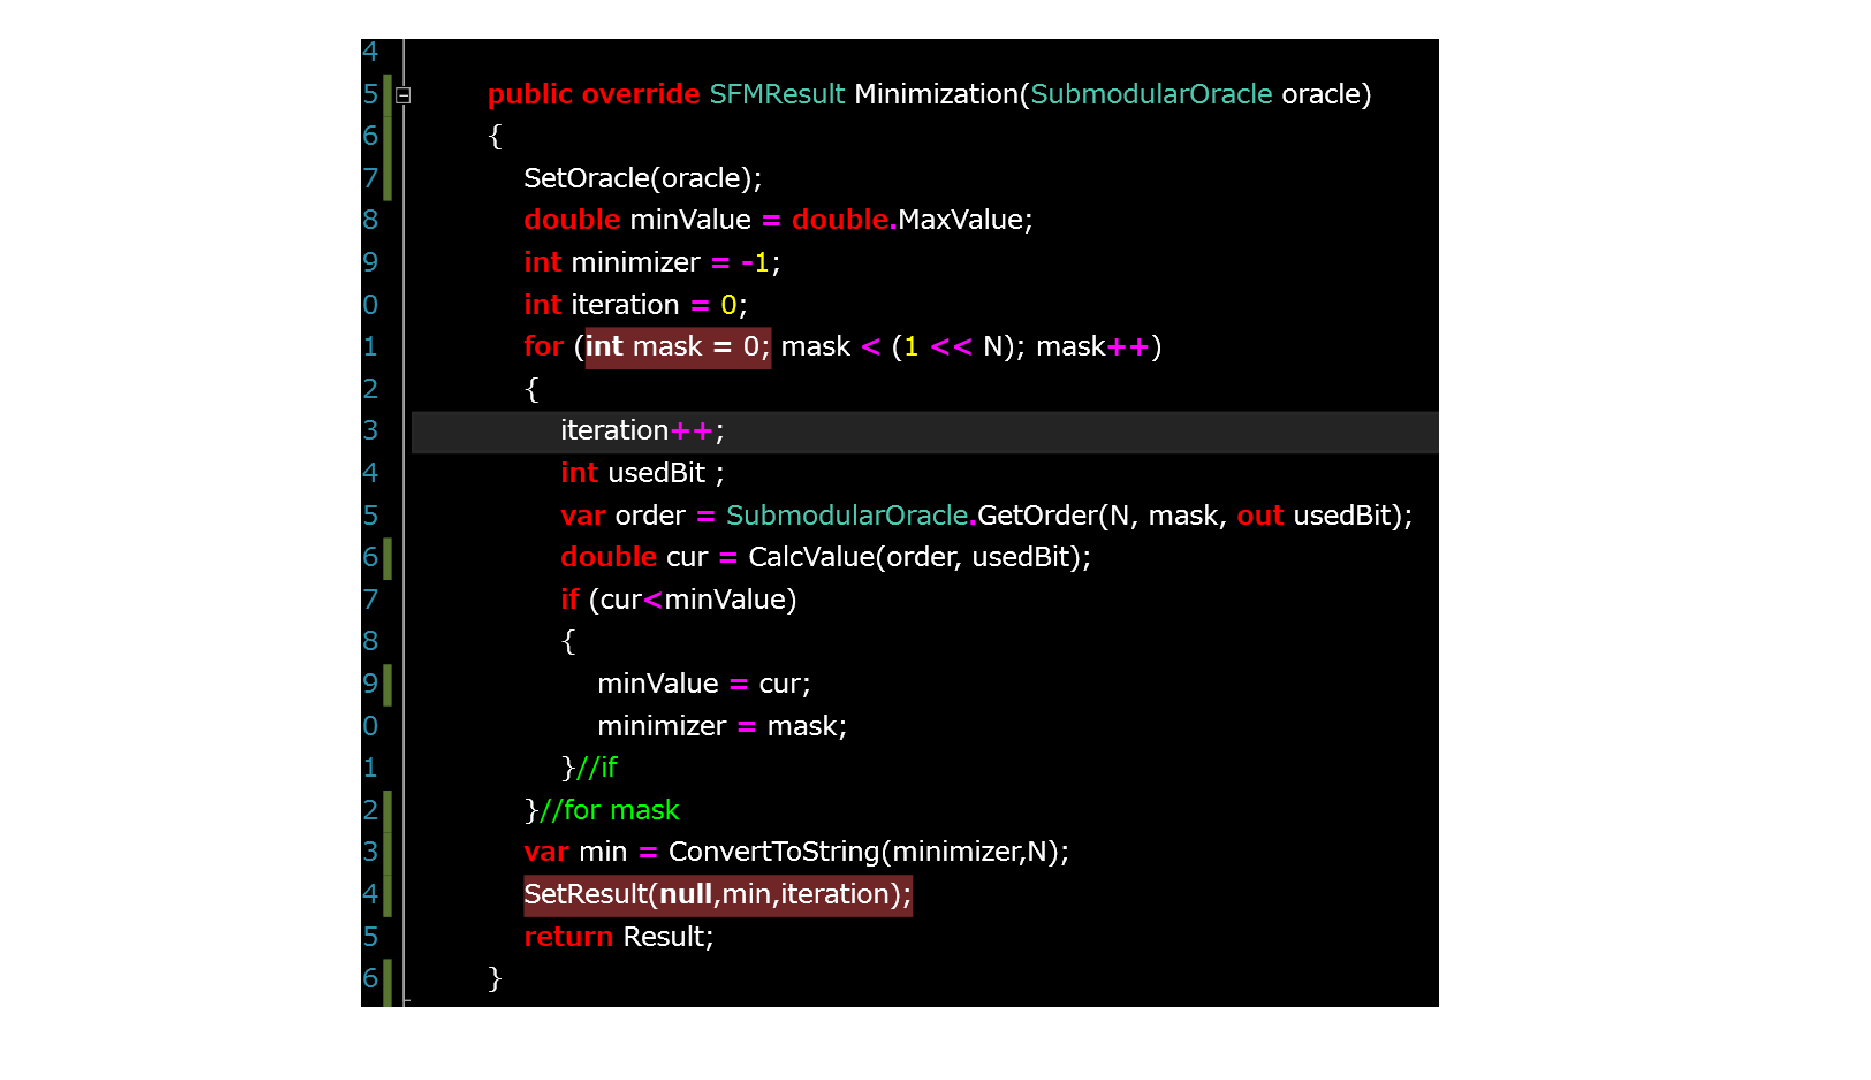
\includegraphics[height=7.0cm]{picture/C++Minimization.png}
\caption{The implementation for Minimization() by a brute force algorithm by C++}
}
\end{figure*}

\begin{figure*}[h!]\label{CSMin}
{
\fontsize{10pt}{12pt}\selectfont
\centering
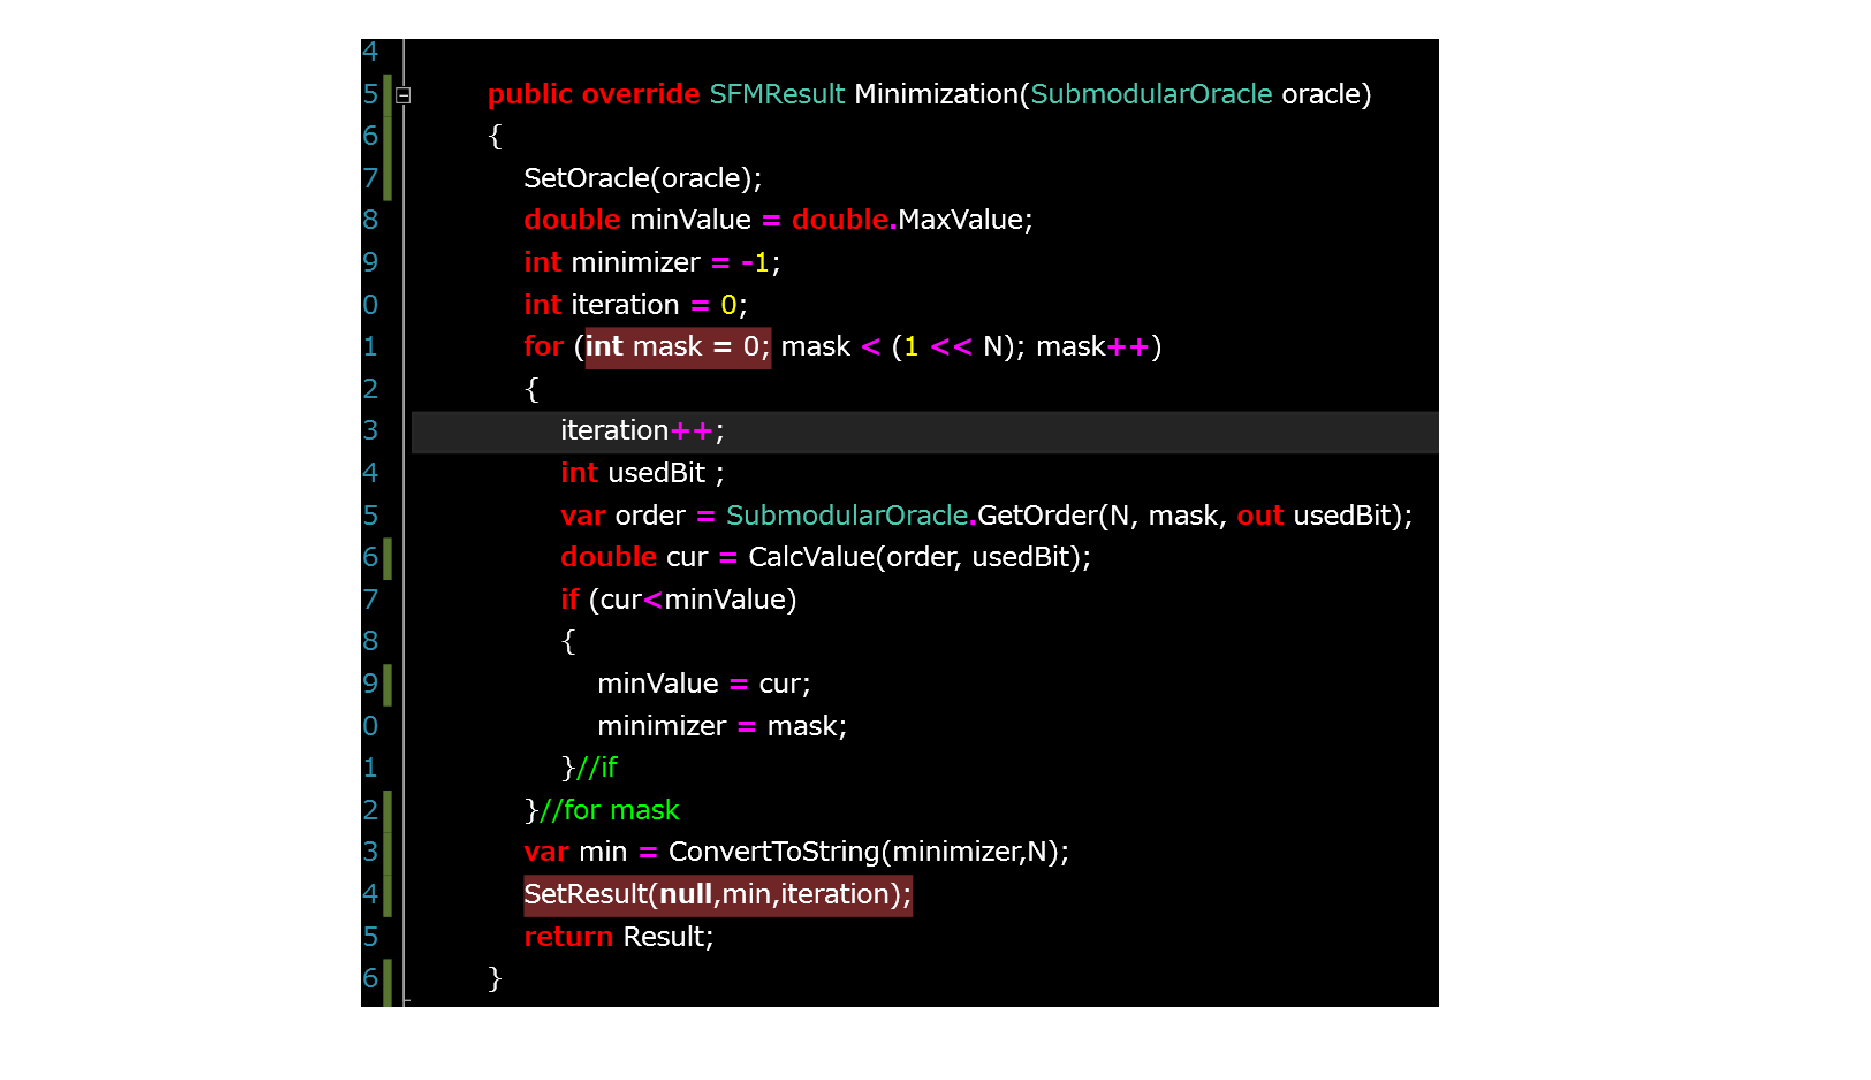
\includegraphics[height=7.0cm]{picture/CSMinimization.png}
\caption{The implementation for Minimization() of a brute force algorithm by C\#}
}
\end{figure*}









\bibliography{sfo.bib}


\end{document} 
